%----------------------------------------------------------------------------------------
%	PACKAGES AND THEMES
%----------------------------------------------------------------------------------------
\documentclass[aspectratio=169,xcolor=dvipsnames]{beamer}
\usetheme{Simple}
\usepackage[backend=bibtex,
defernumbers=true,
style=numeric,
citestyle=ieee
]{biblatex}
\addbibresource{ref.bib}
\usepackage{hyperref}
\graphicspath{{./images/}}
\usepackage{graphicx} % Allows including images
\usepackage{booktabs} % Allows the use of \toprule, \midrule and \bottomrule in tables
\usepackage[utf8]{inputenc}
\usepackage[T1]{fontenc}
\usepackage{amsmath,amssymb}
\usepackage{multirow}
\usepackage{array}


% Uncomment here for a Turkish presentation.
%\AtBeginDocument{%
%	\renewcommand\tablename{Tablo}
%}
%\AtBeginDocument{%
%	\renewcommand\figurename{Şekil}
%}

%----------------------------------------------------------------------------------------
%	TITLE PAGE
%----------------------------------------------------------------------------------------

% The title
\title[Title]
{
	Presentation Title
}

\subtitle{Subtitle}
\author[GTU]{Student: John SMITH  \and
	 Project Advisor: Dr.Beth ADVISOR }

% can specify the institute here
%\institute[]{\inst{1}Bilgisayar Mühendisliği Bölümü\\Gebze Teknik Üniversitesi\and\inst{2}Bilişim Teknolojileri Enstitüsü\\Gebze Teknik Üniversitesi}

\date{\today} % Date, can be changed to a custom date


%----------------------------------------------------------------------------------------
%	PRESENTATION SLIDES
%----------------------------------------------------------------------------------------

\begin{document}

\begin{frame}
    % Print the title page as the first slide
    \titlepage
\end{frame}


% Uncomment here if you want a table of contents. You should use \section etc. (explained below)
% \begin{frame}{Preface}
%     % Throughout your presentation, if you choose to use \section{} and \subsection{} commands, these will automatically be printed on this slide as an overview of your presentation
%     \tableofcontents
% \end{frame}


%------------------------------------------------

\begin{frame}{The Problem}
	This is an unofficial template. The layout of contents might not match with the requirements. This template is shared to provide a quick start to latex presentations in GTU. Here are some items to list:\\
	\vspace{0.03\textheight} % some tweak to add space
	\begin{itemize}
		\item Item 1
		\item Item 2
		\item Item 3
	\end{itemize}
	\vspace{0.03\textheight} % some tweak to add space
	Some text to conclude the list.
\end{frame}

%------------------------------------------------

\begin{frame}{Project Design Plan}
	In this slide, some important text will be \alert{highlighted} because it's important. Please, don't abuse it.
	
	\begin{block}{Block}
		Sample text
	\end{block}
	
	\begin{alertblock}{Alertblock}
		Sample text in red box
	\end{alertblock}
	
	\begin{examples}{Example}
		Sample text in green box. The title of the block is ``Examples".
	\end{examples}
\end{frame}

%------------------------------------------------


%------------------------------------------------

\begin{frame}{Citing and Figures}
	You can cite like this as index \cite{redmon2016look} or you can cite the authors \citeauthor{redmon2016look}. All you need to do is add the citation in BibTeX format to the \textbf{ref.bib} file. Check this \cite{bib} for more.
	
	
	\begin{figure}
		\centering
		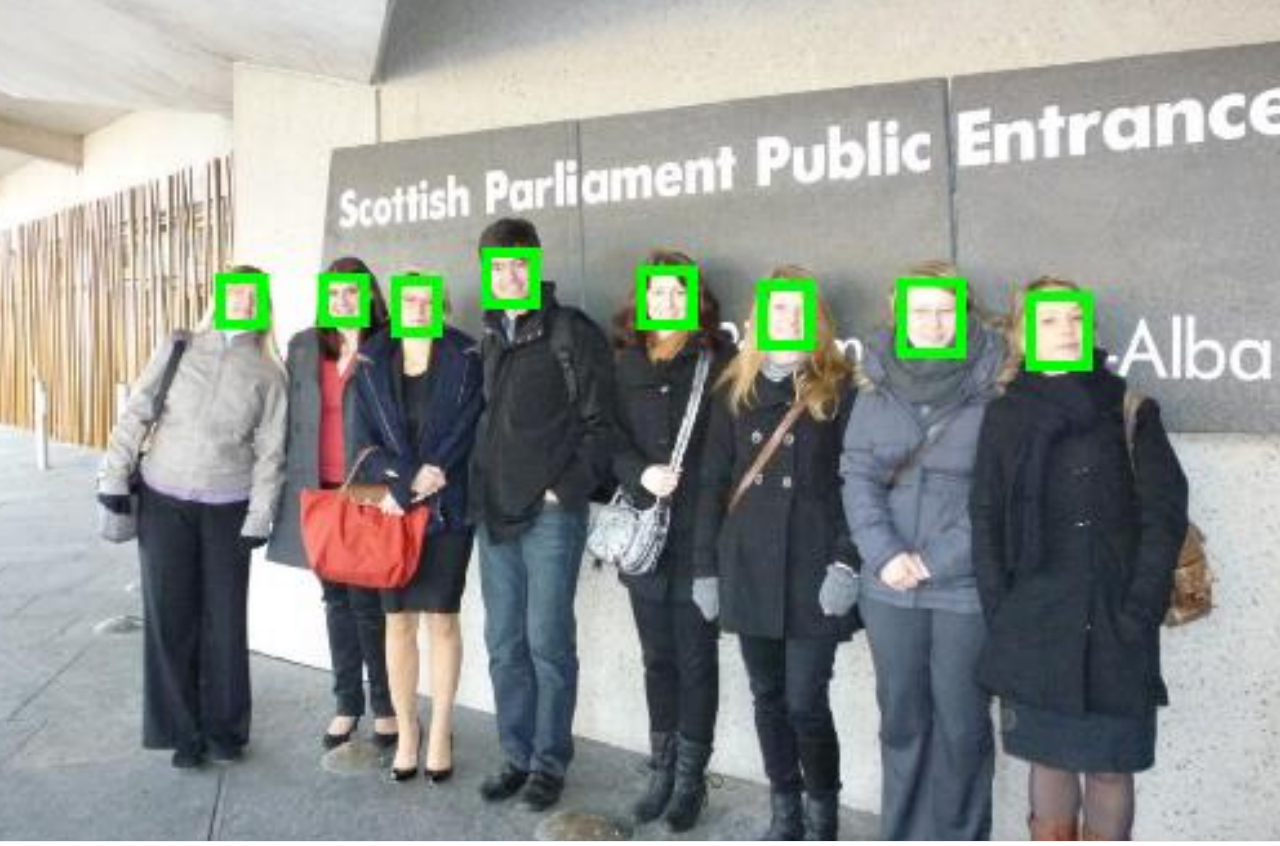
\includegraphics[width=0.4\linewidth]{images/widerface}
		\caption{Caption to this unrelated image}
		\label{fig:widerface}
	\end{figure}
	
\end{frame}

%------------------------------------------------
\begin{frame}{Requirements}
	\begin{columns}[c] % The "c" option specifies centered vertical alignment while the "t" option is used for top vertical alignment
		
		\column{.45\textwidth} % Left column and width
		\textbf{Heading}
		\begin{enumerate}
			\item Statement
			\item Explanation
			\item Example
		\end{enumerate}
		
		\column{.5\textwidth} % Right column and width
		Lorem ipsum dolor sit amet, consectetur adipiscing elit. Integer lectus nisl, ultricies in feugiat rutrum, porttitor sit amet augue. Aliquam ut tortor mauris. Sed volutpat ante purus, quis accumsan dolor.
		
	\end{columns}
\end{frame}

%------------------------------------------------


%------------------------------------------------
\begin{frame}{Success Criteria}
	\begin{table}
		\begin{tabular}{l l l}
			\toprule
			\textbf{Treatments} & \textbf{Response 1} & \textbf{Response 2} \\
			\midrule
			Treatment 1         & 0.0003262           & 0.562               \\
			Treatment 2         & 0.0015681           & 0.910               \\
			Treatment 3         & 0.0009271           & 0.296               \\
			\bottomrule
		\end{tabular}
		\caption{Table caption}
	\end{table}
\end{frame}

%------------------------------------------------

\begin{frame}{Success Criteria Metrics}
	\begin{theorem}[Mass--energy equivalence]
		$E = mc^2$
	\end{theorem}
	\begin{equation}
		MAE=\frac{1}{n}\sum_{i=1}^{n}|c_i- \hat{c}_i|
	\end{equation} 
	\begin{equation}
		RMSE=\sqrt{\frac{1}{n}\sum_{i=1}^{n}(c_i - \hat{c}_i)^2}
	\end{equation}
\end{frame}

%------------------------------------------------

\begin{frame}[allowframebreaks]{References}
    % This might take more than one page
    \printbibliography
\end{frame}

%------------------------------------------------

\begin{frame}
    \Huge{\centerline{Thanks}}
\end{frame}

%------------------------------------------------

	

\end{document}